
%=========================================================
\begin{figure}[t]
\centering
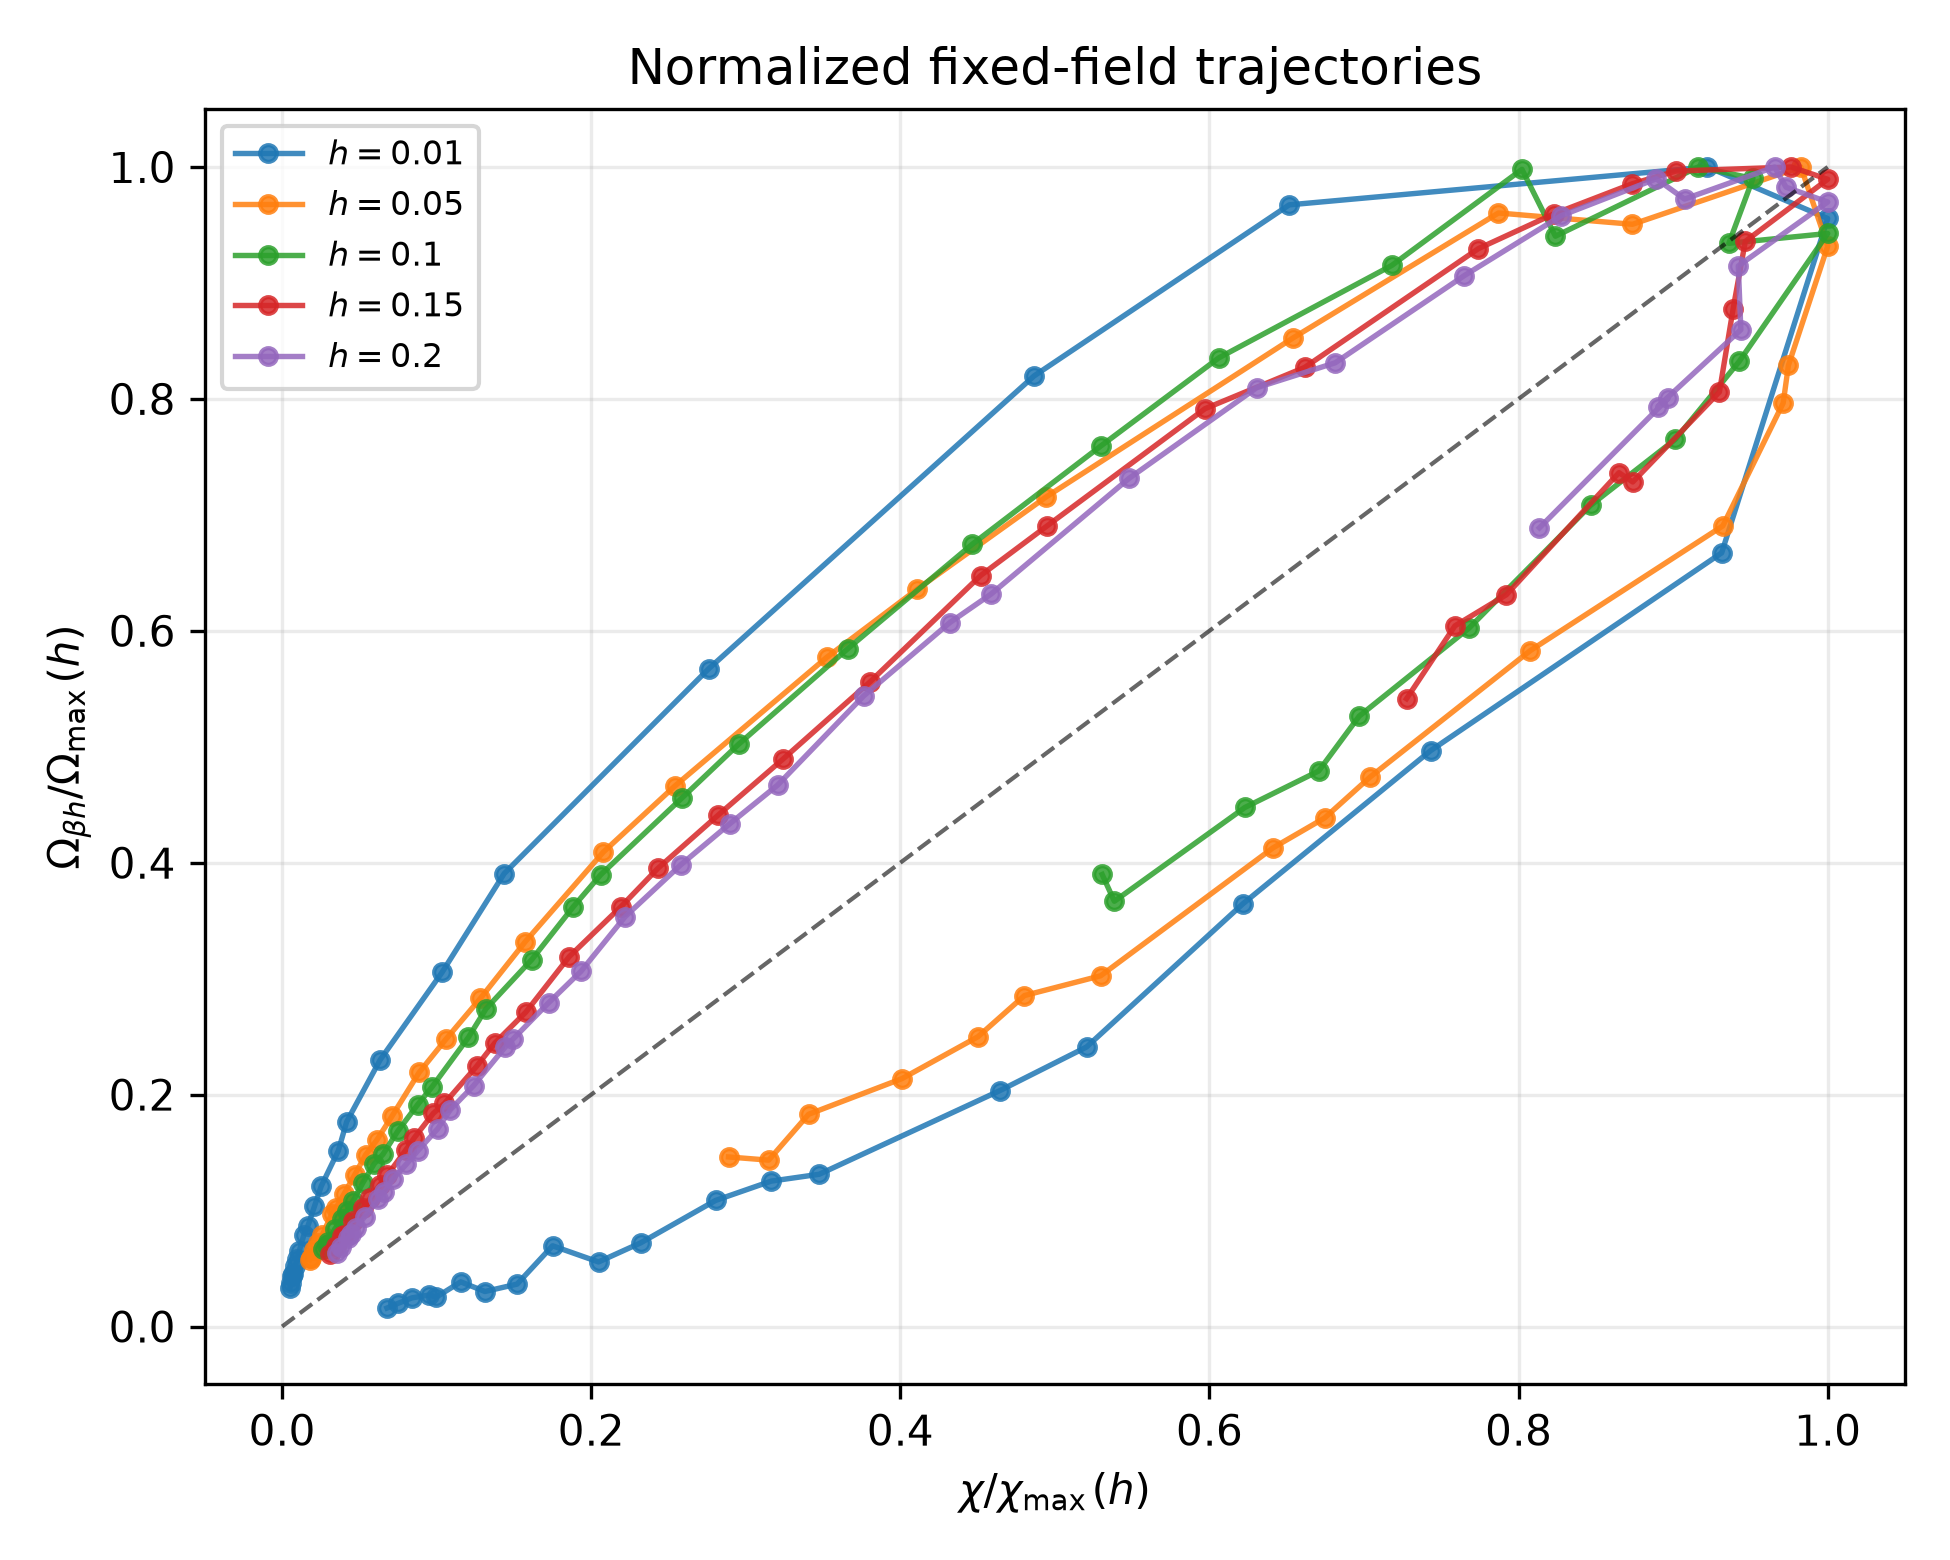
\includegraphics[width=\columnwidth]{Figures/omega_vs_chi_normalized_trajectories.png}
\caption{
Emergent response manifold in the two-dimensional Ising model.
Trajectories obtained for different values of the external
field are represented in terms of the normalized response
coordinates
\(\tilde{\chi}=\chi_T/\chi_{T,\mathrm{max}}\)
and
\(\tilde{\Omega}=\Omega_{Th}/\Omega_{Th,\mathrm{max}}\).
Despite corresponding to distinct thermodynamic trajectories
in the control manifold, the normalized responses collapse
onto an approximately universal curve. The result indicates
that the susceptibility and mixed response are not independent
observables but are constrained by an emergent geometric
relationship. The collapse provides evidence that the image of
the two-dimensional control manifold is concentrated near a
lower-dimensional object in response space, suggesting the
existence of an underlying response manifold that organizes
thermodynamic behavior across a broad range of temperatures
and fields.
}
\label{fig:response_manifold}
\end{figure}
%=========================================================